51. а) $y=-|x^2-2x|=\begin{cases} 2x-x^2,\ x\leqslant0,\\ x^2-2x,\ 0<x<2,\\ 2x-x^2.\ x\geqslant2.\end{cases}$
$$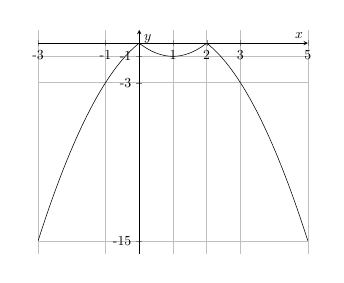
\begin{tikzpicture}[scale=0.5]
\begin{axis}[
    axis lines = middle,
    grid=major,
    legend pos={south west},
    xlabel = {$x$},
    %xlabel style={below right},
    ylabel = {$y$},
    ymin=-16,
    ymax=1,
    xmin=-3,
    xmax=5,
    xtick={-3,-1,1,2,3,5},
    xticklabels={-3,-1,1,2,3,5},
    ytick={ -15,-3,-1},
    yticklabels={ -15,-3,-1},
                  ]
	\addplot[domain=-3:5, samples=100, color=black] {-abs(x*x-2*x)};
   % \addplot[domain=-3:3, samples=100, color=black] {-x};
     %\addlegendentry{$\text{Рис. 1}$};
\end{axis}
\end{tikzpicture}$$
б) По графику найдём $a\in(-\infty;-1)\cup\{0\}.$\\
